%----------------------------------------------------------------------------------------
%	PACKAGES AND OTHER DOCUMENT CONFIGURATIONS
%----------------------------------------------------------------------------------------

\documentclass{article}

\usepackage[utf8]{inputenc}
\usepackage{amssymb}
\usepackage{clrscode3e}
\usepackage{bbm}
\usepackage{amsmath}
\usepackage{float}
\usepackage{latexsym}
\usepackage{subcaption}
\usepackage{gensymb}
\usepackage{caption}
\usepackage{fancyhdr} % Required for custom headers
\usepackage{lastpage} % Required to determine the last page for the footer
\usepackage{extramarks} % Required for headers and footers
\usepackage[usenames,dvipsnames]{color} % Required for custom colors
\usepackage{graphicx} % Required to insert images
\usepackage{listings} % Required for insertion of code
\usepackage{courier} % Required for the courier font
\usepackage{lipsum} % Used for inserting dummy 'Lorem ipsum' text into the template
\usepackage{tabularx} % For nice tables

%%%% NEW
\usepackage{color}

\definecolor{mygreen}{rgb}{0,0.6,0}
\definecolor{mygray}{rgb}{0.5,0.5,0.5}
\definecolor{mymauve}{rgb}{0.58,0,0.82}

\lstset{ %
  backgroundcolor=\color{white},   % choose the background color; you must add \usepackage{color} or \usepackage{xcolor}
  basicstyle=\footnotesize,        % the size of the fonts that are used for the code
  breakatwhitespace=false,         % sets if automatic breaks should only happen at whitespace
  breaklines=true,                 % sets automatic line breaking
  captionpos=b,                    % sets the caption-position to bottom
  commentstyle=\color{mygreen},    % comment style
  deletekeywords={...},            % if you want to delete keywords from the given language
  escapeinside={\%*}{*)},          % if you want to add LaTeX within your code
  extendedchars=true,              % lets you use non-ASCII characters; for 8-bits encodings only, does not work with UTF-8
  frame=single,	                   % adds a frame around the code
  keepspaces=true,                 % keeps spaces in text, useful for keeping indentation of code (possibly needs columns=flexible)
  keywordstyle=\color{blue},       % keyword style
  language=Octave,                 % the language of the code
  otherkeywords={*,...},           % if you want to add more keywords to the set
  numbers=left,                    % where to put the line-numbers; possible values are (none, left, right)
  numbersep=5pt,                   % how far the line-numbers are from the code
  numberstyle=\tiny\color{mygray}, % the style that is used for the line-numbers
  rulecolor=\color{black},         % if not set, the frame-color may be changed on line-breaks within not-black text (e.g. comments (green here))
  showspaces=false,                % show spaces everywhere adding particular underscores; it overrides 'showstringspaces'
  showstringspaces=false,          % underline spaces within strings only
  showtabs=false,                  % show tabs within strings adding particular underscores
  stepnumber=2,                    % the step between two line-numbers. If it's 1, each line will be numbered
  stringstyle=\color{mymauve},     % string literal style
  tabsize=2,	                   % sets default tabsize to 2 spaces
  title=\lstname                   % show the filename of files included with \lstinputlisting; also try caption instead of title
}


%%%% NEW

% Margins%
\topmargin=-0.45in
\evensidemargin=0in
\oddsidemargin=0in
\textwidth=6.5in
\textheight=9.0in
\headsep=0.25in

\linespread{1.1} % Line spacing
%%%
% Set up the header and footer
\pagestyle{fancy}
\lhead{Machine Learning - Assignment 2} % Top left header
\chead{}
\lfoot{\lastxmark} % Bottom left footer
\cfoot{} % Bottom center footer
\rfoot{Page\ \thepage} % Bottom right footer
\renewcommand\headrulewidth{0.4pt} % Size of the header rule
\renewcommand\footrulewidth{0.4pt} % Size of the footer rule
\newcommand{\Lagr}{L}

\setlength\parindent{16pt} % Removes all indentation from paragraphs

\setcounter{secnumdepth}{0} % Removes default section numbers


\definecolor{MyDarkGreen}{rgb}{0.0,0.4,0.0} % This is the color used for comments
\lstloadlanguages{SQL} % Load Perl syntax for listings, for a list of other languages supported see: ftp://ftp.tex.ac.uk/tex-archive/macros/latex/contrib/listings/listings.pdf
\lstset{language=SQL, % Use Perl in this example
        frame=single, % Single frame around code
        basicstyle=\small\ttfamily, % Use small true type font
        keywordstyle=[1]\color{Blue}\bf, % Perl functions bold and blue
        keywordstyle=[2]\color{Purple}, % Perl function arguments purple
        keywordstyle=[3]\color{Blue}\underbar, % Custom functions underlined and blue
        identifierstyle=, % Nothing special about identifiers
        commentstyle=\usefont{T1}{pcr}{m}{sl}\color{MyDarkGreen}\small, % Comments small dark green courier font
        stringstyle=\color{Purple}, % Strings are purple
        showstringspaces=false, % Don't put marks in string spaces
        tabsize=5, % 5 spaces per tab
        %
        % Put standard Perl functions not included in the default language here
        morekeywords={rand},
        %
        % Put Perl function parameters here
        morekeywords=[2]{on, off, interp},
        %
        % Put user defined functions here
        morekeywords=[3]{test},
       	%
        morecomment=[l][\color{Blue}]{...}, % Line continuation (...) like blue comment
        numbers=left, % Line numbers on left
        firstnumber=1, % Line numbers start with line 1
        numberstyle=\tiny\color{Blue}, % Line numbers are blue and small
        stepnumber=5 % Line numbers go in steps of 5
}

% Creates a new command to include a perl script, the first parameter is the filename of the script (without .pl), the second parameter is the caption
\newcommand{\perlscript}[2]{
\begin{itemize}
\item[]\lstinputlisting[caption=#2,label=#1]{#1.sql}
\end{itemize}
}


%----------------------------------------------------------------------------------------
% TITLE PAGE
%----------------------------------------------------------------------------------------

\title{
\vspace{1in}
\textmd{\textbf{Machine Learning - Assignment 2}} \\
%\textmd{Assignment 2 - Resubmission} \\
\author{Christoffer Thrysøe - dfv107}
}

%----------------------------------------------------------------------------------------

\begin{document}
\maketitle
% \tableofcontents
\pagenumbering{arabic}
\section{1. K-Nearest Neighbours}
The function \texttt{main()}, found in the file \texttt{KNN.py} can be run to reproduce the results for this assignment.
\subsection{Question: 1.1}
The implemented K-Nearest Neighbour method is located in the file \texttt{KNN.py}. The method works by calculating the euclidean distance, for each input point, to the rest of the points in the data. These distances are then sorted in ascending order and the top $k$ distances are retrieved. Each of these points have a target value, which counts as votes toward a prediction. The target value with the most votes is returned as the predictive class.
\\
To measure the performance of the classifier, the zero-one loss function is used, resulting in 0 if the predicted value $Y'$ is equal to the true target value $Y$ and 1 otherwise:
\begin{equation*}
\begin{split}
\ell(Y',Y) =
\mathbbm{1} \lbrace Y'= Y \rbrace =
\begin{cases}
0,& \textsl{if } Y' = Y  \\
1,&  \textsl{otherwise}
\end{cases}
\end{split}
\label{indikator}
\end{equation*}
The loss will be calculated in respect to the amount of prediction made $N$, that is the average loss. The empirical loss is defined as followed:
\begin{equation*}
\hat{L}(h) =  \dfrac{1}{N}\sum\limits^{N}_{n=1} \ell (h(x_n),y_n)
\end{equation*}
The implemented method is applied to both the training data \texttt{IrisTrainML.dt} and the testing data: \texttt{IrisTestML.dt}, each with values of $k \in \lbrace 1,3,5 \rbrace$.
\\
The below table shows the results of running the aforementioned experiments.
\begin{table}[H]
  \centering
  \label{tab:table1}
  \begin{tabular}{c||c|c}
    \textsf{k} & \textsf{Test} & \textsf{Train} \\
    \hline
    1 & $0.18$ & $0.0$ \\
    3 & $0.18$ & $0.14$ \\    
    5 & $0.31$ & $0.17$\\
  \end{tabular}
  \caption{Empirical loss when running the KNN classifier on the testing and training set for different values of k} 
\end{table}
Note from table \ref{tab:table1} that the empirical loss of $k=1$ on the training data, is always zero as the closest neighbour of a given point is always the point itself. The test data is treated as unknown values in the training set, therefore the empirical loss of $k=1$ is not 0, as the entry doesn't exist in the data set.
\subsection{Question 1.2}
Cross validation is used for the K-Nearest Neighbour algorithm, in order to find the best suited value of $k$. The applied validation is a \textit{5-fold cross validation}, which means that the dataset is split into 5 equal sized partitions, where for a fixed k, one of these partitions is used as a validation set. This is performed for each fold, thus 5 times. The average loss of these five folds is used to estimate the performance of the classifier. These folds are performed for $k \in \lbrace 1,3,5,...,25 \rbrace$ in order to find the value $k$, which results in the lowest average loss, this choosing of $k$ will be denoted as $k_{best}$.  
The 5-fold validation is implemented in the function called \texttt{crossValidate} located in the file \texttt{KNN.py}. The method works by creating a random permutation of the input data, this permutation is then split into 5 equally sized partitions. The validation algorithm is then run for each value of $k$ and each partition.
\begin{figure}[H]
  \centering
  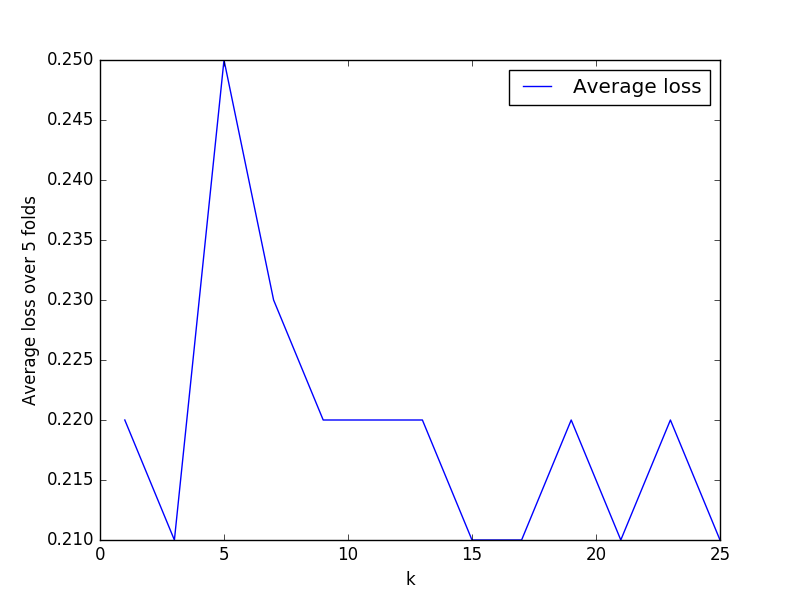
\includegraphics[width=10cm]{ass1.png}
  \caption{Average loss over 5 folds as a function of the values of k}
  \label{fig:cross1}
\end{figure}
The value of k with the lowest 0-1 error is $k = 3 = k_{best}$
The generalization performance of $k_{best}$ is found evaluating the 3-KNN classifier on the test data. The general performance of 3-KNN is $0.18$.
\\ The result of the cross validation was somewhat surprising as i would have thought that the larger the k, the bigger the loss. However as evident in figure \ref{fig:cross1} there is no direct connection between the size of $k$ and the loss. Also when running the cross validation multiple times, with different random partitions, the value of $k_{best}$ would change. $k=3$, has been chosen as $k_{best}$ as it more often than not, provides the lowest cost, when performing cross validation. Table \ref{tab:table2} shows the empirical loss from running the classifier on the training and testing data sets, with $k = k_{best} = 3$:
\begin{table}[H]
  \centering
  \label{tab:table2}
  \begin{tabular}{c||c|c}
    \textsf{k} & $\textsl{Test}$ & $\textsl{Train}$\\
    \hline
    \textsl{3} & $0.18$ & $0.14$ \\
  \end{tabular}
  \caption{Empirical loss when running the KNN classifier on the testing and training set with $k=3$} 
\end{table}
\subsection{Question 1.3}
The objective of the normalization procedure is to perform a zero-mean, unit variance transformation on the input data. To do so, we apply a linear mapping from the input data to the normalized output data. Thus we wish to determine some  $t$:
\begin{equation}
X_{norm}=t(X)
\end{equation}
such that $\mu(X_{norm})=0$ and $Var(X_{norm})=1$ \\
To achieve this, the mean of each input feature is found and subtracted. The mean is calculated by:
\begin{equation*}
\mu(X) = \dfrac{1}{N} \sum\limits^{N}_{i=1}x_i
\end{equation*}
 Next the variance is found of each feature. The variance is calculated by:
\begin{equation*}
Var(X) = \dfrac{1}{N} \sum\limits^{N}_{i=1}(x_i - \mu)^2
\end{equation*}
The standard deviation $\sigma$ is equal to the square root of the variance and is used to normalize the data. The normalization can then be expressed as the following:
\begin{equation}
X_{norm} = \dfrac{X - \mu(X) }{\sigma}
\label{norm}
\end{equation}
Thus defining the linear mapping from $X$ to $X_{norm}$. Below is the mean and variance for the training data \texttt{IrisTrainML.dt} and the normalized test data \texttt{IrisTestML.dt}. The mean and variance of the training data is used to normalize the test data, using equation \eqref{norm} \\
\begin{table}[H]
  \centering
  \label{tab:table3}
  \begin{tabular}{c||c|c}
    \textsf{ } & \textsl{Training} & \textsl{$Test_{norm}$} \\
    \hline
    \textsl{Mean} & $(5.75,0.3)$ & $(0.20,0.43)$ \\
    \textsl{Variance} & $(0.6888,0.0017)$ & $(1.07,1.25)$ \\    
  \end{tabular}
  \caption{Left: Mean and Variance calculated on the training data. Right: The Mean and Variance of the data which has been normalized using the values for mean and variance in the left column.} 
\end{table}
The variance and mean for the normalized test data is slightly larger than of the training data.
\\
Running the cross validation algorithm on normalized data yields the following results:
\begin{figure}[H]
  \centering
  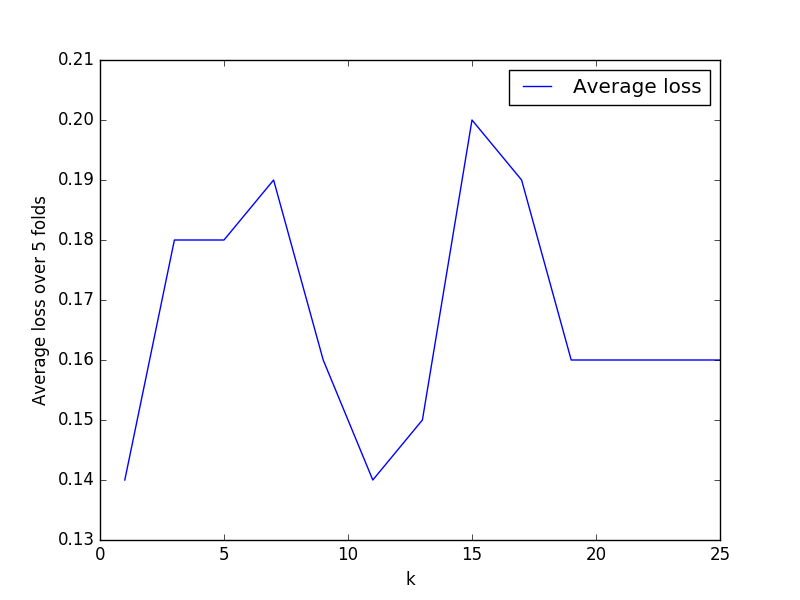
\includegraphics[width=10cm]{ass12.png}
  \caption{Average loss over 5 folds as a function of the values of k, found using the normalized data.}
  \label{fig:fig1}
\end{figure}
The above results suggests a $k_{best} = 1 \textsl{ or } 11$, as in the cross validation for non-normalized data the the result is contra distinctive. A clear difference from the results of running the cross validation on non-normalized data and on normalized data is that the normalized data produce a much smaller loss.
\begin{table}[H]
  \centering
  \label{tab:table4}
  \begin{tabular}{c||c|c}
    \textsf{k} & $\textsl{Test}$ & $\textsl{Train}$\\
    \hline
    \textsl{1} & $0.18$ & $0.0$ \\
    \textsl{11} & $ 0.42 $ & $ 0.23 $ \\    
  \end{tabular}
  \caption{Empirical loss when running the KNN classifier on the testing and training set for different values of k} 
\end{table}
This feature normalization is performed to ensure that each feature counts equally. Features are measured on different scales, for example some features may range big values where others small. To ensure that features count equally they are scaled to lie in the same range. This is essential when dependent on distance metrics as non-normalized data can create a huge bias toward one feature. I believe the improved results of the cross validation, performed on normalized data, is due to the normalization of the data, and the removal of potential bias in the data.
\section{2 Markov's inequality vs. Hoeffding's inequality vs. binomial bound}
\subsection{1}
To bound the probability using markov's inequality, the expected value of $S$ is determined:\\
\begin{equation*}
\mathbb{E}[S] = \mathbb{E} \left[\sum\limits^{10}_{i=1}X_i\right] = \sum\limits^{10}_{i=1} \mathbb{E}[X_i]
\end{equation*}
The expected value of the Bernoulli random variable with bias = $\frac{1}{2}$ is defined as followed:
\begin{equation*}
\mathbb{E}[X] = Pr[X=1] \times 1 + Pr[X=0] \times 0 = \dfrac{1}{2}
\end{equation*}
the expected value of $S$ is:
\begin{equation*}
\mathbb{E}[S]= \left[\sum\limits^{10}_{i=1}X_i\right] = 10 \times \dfrac{1}{2} = 5
\end{equation*}
therefore the inequality can be written as followed:
\begin{equation*}
Pr[S \geq 9] \leq \dfrac{\mathbb{E}[S]}{9} = \dfrac{5}{9} \approx 0.55
\end{equation*}
\subsection{2}
Given the independence of the variables and that $ \mathbb{E}[X_i] = \mu $
Hoeffding's inequality can be defined as:
\begin{equation*}
Pr\left[ \dfrac{1}{n} \sum\limits^{n}_{i=1}X_i - \mu \geq \epsilon \right]
\leq e^{-2n\epsilon^2}
\end{equation*}
which can be rewritten as:
\begin{equation*}
Pr\left[ \dfrac{1}{n} \sum\limits^{n}_{i=1}X_i \geq n(\mu + \epsilon) \right]
\leq e^{-2n\epsilon^2}
\end{equation*}
noting that, $n=10$, $\mu= \dfrac{1}{2}$ solving for $\epsilon$ in\\
$$ 10(\epsilon+ \dfrac{1}{2}) \textsl{, yields: } \epsilon=\dfrac{2}{5} $$
the value of epsilon can now be input into the above inequality:
\begin{equation*}
Pr \left[ \sum\limits^{n}_{i=1}X_i \geq 9 \right] \leq e^{-2 \times 10 \times \frac{2}{5}^2} = e^{-\frac{16}{5}}  \approx 0.04
\end{equation*}
\subsection{3}
The probability of $S \geq 9$ is equal to the probability of $Pr[S=9]$ + $Pr[S=10]$ as the events are independent:
\begin{align*}
Pr[S=9] &= \binom{10}{9} \times \dfrac{1}{2}^9 \times \left( 1 - \dfrac{1}{2} \right)^1 = \dfrac{10}{1024} \\
Pr[S=10] &= \binom{10}{10} \times \dfrac{1}{2}^{10} \times \left( 1 - \dfrac{1}{2} \right)^0 = \dfrac{1}{1024} \\
\end{align*}
and therefore the probability is:
\begin{equation*}
Pr[S\geq 9] = \frac{10}{1024} + \frac{1}{1024} = \frac{11}{1024} \approx 0.0107
\end{equation*}
\subsection{4}
The bounded probability using Markov's inequality is very loose compared to the bounded probability by Hoeffding's inequality. The bounded probability using Markov's inequality is about 50 times greater than the exact probability where the bounden probability by Hoeffding's inequality is about 13 times greater than the exact.
\section{3. The effect of scale (range) and normalization of random variables in Hoeffding's inequality}
Corollary 1.4 assumes $ X_1,...,X_n$ are independent, such that $Pr[X_i \in [0,1]] = 1$ and that $\mathbb{E}[X_i]=\mu$. Given the above, we can apply Theorem 1.2 , that is we can express the term as followed $\sum_{i=1}^n (b_i-a_i)^2 = \sum_{i=1}^n (1-0)^2 =
\sum_{i=1}^n 1 = n $. We let $\epsilon' = n\epsilon$ in theorem 1.2 and make use of the above, therefore:
\begin{equation*}
Pr \left[ \sum\limits^n_{i=1} X_i-\mathbb{E} \left[\sum\limits^n_{i=1} X_i \right] \geq \epsilon'\right] \leq e^{ -2 \epsilon'^2 / \sum_{i=1}^n(b_i-a_i)^2  }= e^{-2\epsilon'^2/n}
\end{equation*}
Because of independence we can define:
$\mathbb{E}[\sum_{i = 1}^{n}X_i]= \sum_{i = 1}^{n}\mathbb{E}[X_i] = \sum_{i = 1}^{n} \mu = \mu n $ putting the expected value into the inequality:
\begin{equation*}
Pr \left[ \sum\limits^n_{i=1} X_i - \mu n  \geq \epsilon' \right] \leq e^{-2\epsilon'^2/n}
\end{equation*}
If we now replace $\epsilon'$ with $n\epsilon$, and multiply $\frac{1}{2}$ to get rid of $n$ in the inner term:
\begin{equation*}
Pr \left[ \sum\limits^n_{i=1} X_i - \mu n  \geq n\epsilon' \right] =
Pr \left[ \dfrac{1}{n} \sum\limits^n_{i=1} X_i - \mu  \geq \epsilon \right] 
 \leq e^{-2 n \epsilon^2}
\end{equation*}
thus completing the proof that corollary 1.4 follows from theorem 1.2 for random variables in the $[0,1]$ interval. 
\section{4. Basic Statistics}
\subsection{1}
To bound the probability, i will use Hoeffding's inequality. First we note that for each passenger there is a $\mu = 1-0.05$ change of him/her not showing up. We also note that $n(\mu + \epsilon) = 100$ and $n=100$. As before we solve for $\epsilon$:
$$ 
100(\epsilon + \frac{95}{100}) = 100 \textsl{, yields: } \epsilon = \dfrac{1}{20}
$$
The value for $\epsilon$ can then be inserted into the inequality:
\begin{equation*}
Pr \left[ \sum\limits^{n}_{i=1}X_i \geq 100 \right] \leq e^{-2 \times 100 \times \frac{1}{20}^2} = e^{-\frac{1}{2}}  \approx 0.60
\end{equation*}
\subsection{2}
%https://people.cs.umass.edu/~domke/courses/sml2010/10theory.pdf
\section{5}
The function \texttt{main()}, found in the file \texttt{linregs.py} can be run to produce the results for this assignment.
\subsection{Question 5.1}
\subsubsection{1}
The implemented linear regression algorithm can be found in the file \texttt{linregs.py}. \\
First the data is loaded from the file \texttt{DanWood.dt}, the data is then prepared, that is split into x and y values. The intercept is added for the $\mathbf{X}$, setting $x_0$ to 1. The weights $w$ are then calculated as  $w = (\mathbf{X}^T \mathbf{X})^{-1}\mathbf{X}^T y$. The predictions $\hat{y}$ are estimated as $ \hat{y} = \mathbf{X}w$.
\subsubsection{2}
The linear model for the given data is as followed: 
$$ \hat{y} = 9.489 \times x - 10.426 $$
thus the weights are: $w=[-10.426,9.489]$ \\ The mean squared error is defined as:
\begin{equation*}
RMSE = \sqrt{ \dfrac{1}{N} \sum\limits^{n}_{i=1} (y_i - \hat{y}_i )^2}
\end{equation*}
The RMSE of the linear model performed on the data is $0.0124$
\subsubsection{3}
The below figure shows the data points and the linear model as a function of x.
\begin{figure}[H]
  \centering
  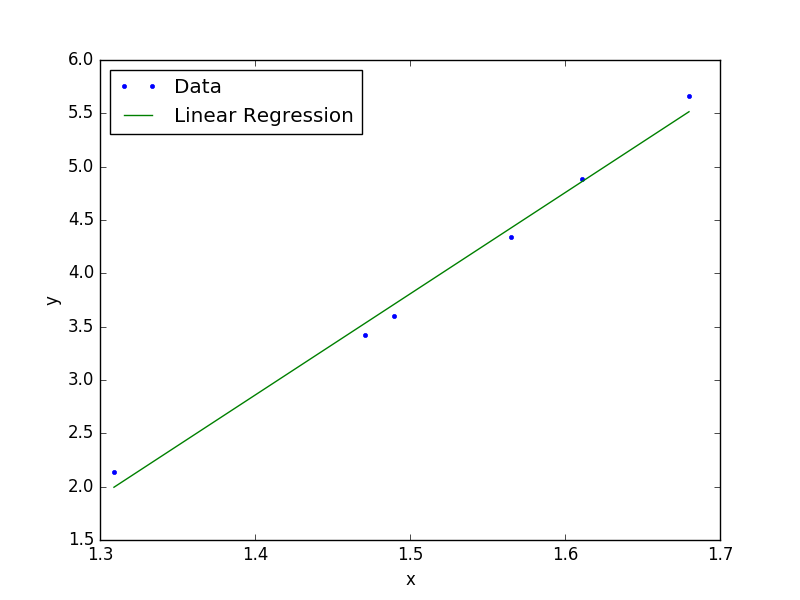
\includegraphics[width=10cm]{ass5.png}
  \caption{Data plotted as points, the linear regression model plotted as a line}
  \label{fig:fig2}
\end{figure}
\subsection{Question 5.2}
Proof that $\mathbf{H} = \mathbf{H}^T $, where $\mathbf{H} = \mathbf{X}(\mathbf{X}^T \mathbf{X})^{-1}\mathbf{X}^T$. A rule used throughout the proof regards the transpose of multiple values and it goes as followed: $ (\mathbf{A} \mathbf{B} \mathbf{C})^T = \mathbf{C}^T \mathbf{B} ^T \mathbf{A}^T  $ , i will refer to this rule as the \textit{transpose rule}. Another rule, which i will refer to as the inverse rule goes as followed: $ (\mathbf{A}^{T})^{-1} = (\mathbf{A}^{-1})^{T} $
\begin{align*}
\mathbf{H} &= \mathbf{X}(\mathbf{X}^T \mathbf{X})^{-1}\mathbf{X}^T \\
\mathbf{H}^T &= \left[\mathbf{X}(\mathbf{X}^T \mathbf{X})^{-1}\mathbf{X}^T \right]^T  \hspace{0.5cm} \textsl{Apply transpose rule to the three inner terms} \\
&= \mathbf{X} \left( (\mathbf{X}^T \mathbf{X})^{-1}\right)^T \mathbf{X}^T \hspace{0.5cm} \textsl{Apply the inverse rule}  \\
&= \mathbf{X} \left( (\mathbf{X}^T \mathbf{X})^{T}\right)^{-1} \mathbf{X}^T \hspace{0.5cm} \textsl{Apply transpose rule to inner term} \\
&= \mathbf{X}  (\mathbf{X}^T \mathbf{X})^{-1}\mathbf{X}^T \\
&= \mathbf{H}
\end{align*}
Thus concluding the proof of $\mathbf{H} = \mathbf{H}^T $
\\
To prove that $\mathbf{H}^k = \mathbf{H}$ i will prove that the matrix is idempotent meaning that $\mathbf{H} \times \mathbf{H} = \mathbf{H}$:
\begin{align}
\mathbf{H}\mathbf{H} &= (\mathbf{X}(\mathbf{X}^T \mathbf{X})^{-1}\mathbf{X}^T) \times (\mathbf{X}(\mathbf{X}^T \mathbf{X})^{-1}\mathbf{X}^T) \\
&= \mathbf{X}(\mathbf{X}^T\mathbf{X})^{-1} (\mathbf{X}^T\mathbf{X})(\mathbf{X}^T\mathbf{X})^{-1} \mathbf{X}^T\\
&= \mathbf{X}(\mathbf{X}^T\mathbf{X})^{-1}  \mathbf{I} \mathbf{X}^T \\
&= \mathbf{X}(\mathbf{X}^T\mathbf{X})^{-1}  \mathbf{X}^T \\
&= \mathbf{H}
\end{align}
where step (4) of the proof uses the property that 
$  (\mathbf{X}^T\mathbf{X})(\mathbf{X}^T\mathbf{X})^{-1} = \mathbf{I} $ \\
Thus concluding the proof of $\mathbf{H} \times \mathbf{H} = \mathbf{H}$, note that this also imply that $\mathbf{H}^k = \mathbf{H}$.

\end{document}
